\documentclass{article}
\usepackage[utf8]{inputenc}

\title{Homework 2}
\author{Benny Chen}
\date{September 20, 2022}

\usepackage{color}
\usepackage{amsthm}
\usepackage{amssymb} 
\usepackage{amsmath}
\usepackage{listings}
\usepackage{xcolor}
\usepackage{listings}
\usepackage{graphicx}
\usepackage{tabularx}
\usepackage[hidelinks]{hyperref}

\lstdefinelanguage[mips]{Assembler}{%
  % so listings can detect directives and register names
  alsoletter={.\$},
  % strings, characters, and comments
  morestring=[b]",
  morestring=[b]',
  morecomment=[l]\#,
  % instructions
  morekeywords={[1]abs,abs.d,abs.s,add,add.d,add.s,addi,addiu,addu,%
    and,andi,b,bc1f,bc1t,beq,beqz,bge,bgeu,bgez,bgezal,bgt,bgtu,%
    bgtz,ble,bleu,blez,blt,bltu,bltz,bltzal,bne,bnez,break,c.eq.d,%
    c.eq.s,c.le.d,c.le.s,c.lt.d,c.lt.s,ceil.w.d,ceil.w.s,clo,clz,%
    cvt.d.s,cvt.d.w,cvt.s.d,cvt.s.w,cvt.w.d,cvt.w.s,div,div.d,div.s,%
    divu,ecall,eret,floor.w.d,floor.w.s,j,jal,jalr,jr,l.d,l.s,la,lb,lbu,%
    ld,ldc1,lh,lhu,li,ll,lui,lw,lwc1,lwl,lwr,madd,maddu,mfc0,mfc1,%
    mfc1.d,mfhi,mflo,mov.d,mov.s,move,movf,movf.d,movf.s,movn,movn.d,%
    movn.s,movt,movt.d,movt.s,movz,movz.d,movz.s,msub,msubu,mtc0,mtc1,%
    mtc1.d,mthi,mtlo,mul,mul.d,mul.s,mulo,mulou,mult,multu,mulu,mv,neg,%
    neg.d,neg.s,negu,nop,nor,not,or,ori,rem,remu,rol,ror,round.w.d,%
    round.w.s,s.d,s.s,sb,sc,sd,sdc1,seq,sge,sgeu,sgt,sgtu,sh,sle,%
    sleu,sll,sllv,slt,slti,sltiu,sltu,sne,sqrt.d,sqrt.s,sra,srav,srl,%
    srlv,sub,sub.d,sub.s,subi,subiu,subu,sw,swc1,swl,swr,syscall,teq,%
    teqi,tge,tgei,tgeiu,tgeu,tlt,tlti,tltiu,tltu,tne,tnei,trunc.w.d,%
    trunc.w.s,ulh,ulhu,ulw,ush,usw,xor,xori},
  % assembler directives
  morekeywords={[2].align,.ascii,.asciiz,.byte,.data,.double,.extern,%
    .float,.globl,.half,.kdata,.ktext,.set,.space,.text,.word},
  % register names
  morekeywords={[3]\$0,\$1,\$2,\$3,\$4,\$5,\$6,\$7,\$8,\$9,\$10,\$11,%
    \$12,\$13,\$14,\$15,\$16,\$17,\$18,\$19,\$20,\$21,\$22,\$23,\$24,%
    \$25,\$26,\$27,\$28,\$29,\$30,\$31,%
    \$zero,\$at,\$v0,\$v1,\$a0,\$a1,\$a2,\$a3,\$t0,\$t1,\$t2,\$t3,\$t4,
    \$t5,\$t6,\$t7,\$s0,\$s1,\$s2,\$s3,\$s4,\$s5,\$s6,\$s7,\$t8,\$t9,%
    \$k0,\$k1,\$gp,\$sp,\$fp,\$ra},
}[strings,comments,keywords]

\definecolor{CommentGreen}{rgb}{0,.6,0}
\lstset{
  language=[mips]Assembler,
  escapechar=@, % include LaTeX code between `@' characters
  keepspaces,   % needed to preserve spacing with lstinline
  basicstyle=\small\ttfamily\bfseries,
  commentstyle=\color{CommentGreen},
  stringstyle=\color{cyan},
  showstringspaces=false,
  keywordstyle=[1]\color{blue},    % instructions
  keywordstyle=[2]\color{magenta}, % directives
  keywordstyle=[3]\color{red},     % registers
}

\begin{document}

\maketitle

\section*{Question 1}

\begin{center}
    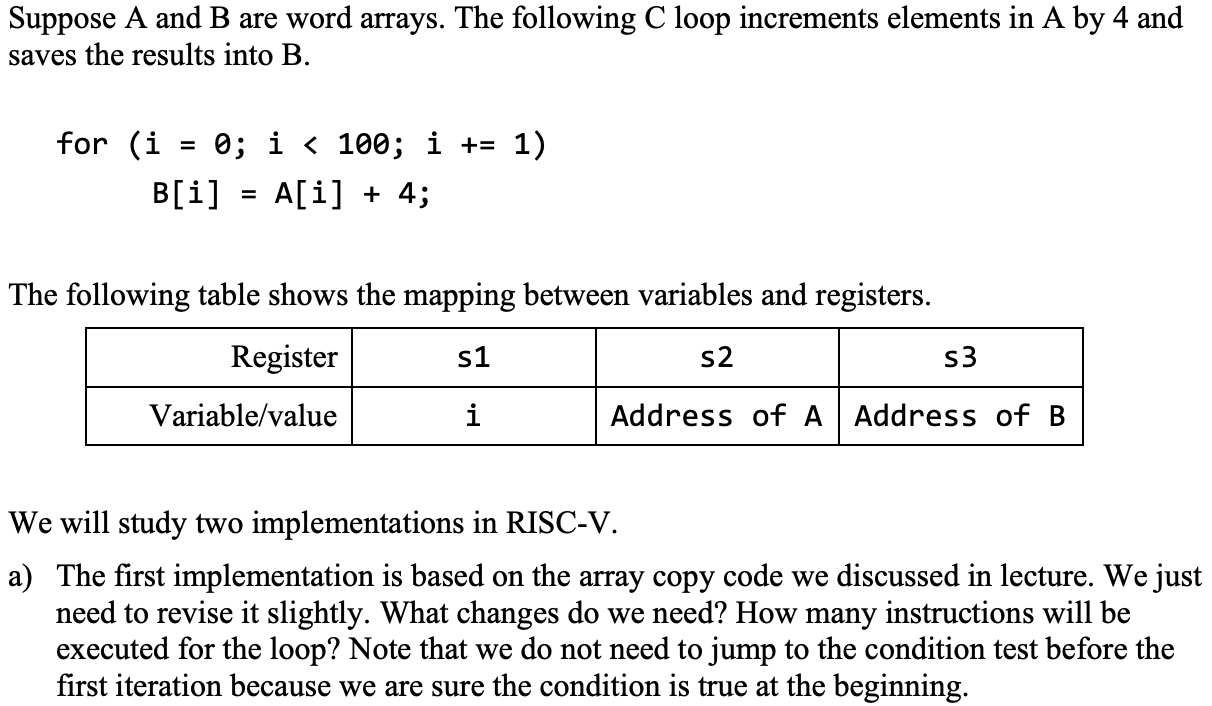
\includegraphics[scale=.56]{./images/q1parta.png}
\end{center}
\subsection*{Part A answer:}

We are already given the bulk of the code from the lectures.
The only change that we would need to make is to add 4 to A[i]
after we load the value to t1. There would be a total of 802 
executed instructions.

\begin{lstlisting}
	addi	s4, x0, 100
	addi	s1, x0, 0
	beq	x0, x0, test # we know s1 < s4
loop:	

	slli	t0, s1, 2 # t0 = i * 4
	add	t2, t0, s2 # compute addr of A[i]
	lw	t1, 0(t2)
	addi	t1,t1,4 # add 4 to A[i]
	add	t3, t0, s3 # compute addr of B[i]
	sw	t1, 0(t3)
	addi	s1, s1, 1

test: 	
	bne	s1, s4, loop # 7 instructions in the loop
\end{lstlisting}

\begin{center}
    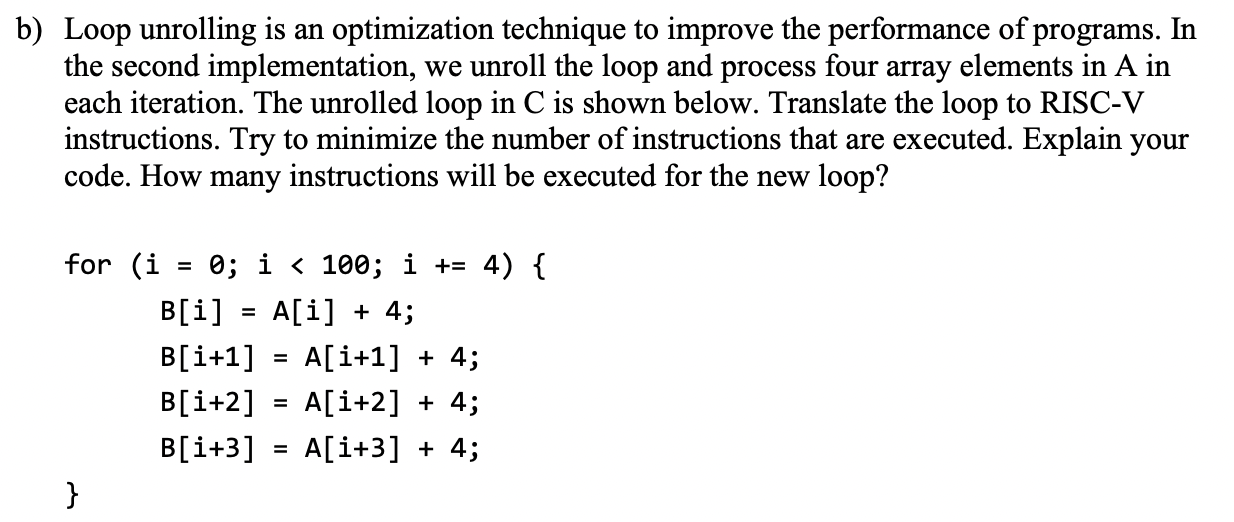
\includegraphics[scale=.557]{./images/q1partb.png}
\end{center}

\subsection*{Part B answer:}
The problem is similar to part A so we can start with a baseline from Part A.
The change for Part B is that we are adding 4 to the index (i) and 
loading 4 values from A[i,i+1,i+2,i+3] to B[i,i+1,i+2,i+3]. Since we know how to 
find the address of A[i] and B[i] we can just add 4 to the address to increment
the index by 1. There would be a total of 427 executed instructions.
\begin{lstlisting}
	addi	s4, x0, 100 #100
	addi	s1, x0, 0 #i = 0
	beq	x0, x0, test # we know s1 < s4
	
loop:	
	#Address calculation
	slli	t0, s1, 2 # t0 = i * 4
	
	# B[i] = A[i] + 4
	add	t2, t0, s2 # compute addr of A[i]
	lw	t1, 0(t2)
	addi	t1,t1,4 # add 4 to A[i]
	add	t3, t0, s3 # compute addr of B[i]
	sw	t1, 0(t3) # load A[i] + 4 to B[i] 
	# We know A[i] and B[i] address so we just need 
	# to load adress + 4 to have A and B [i+1]
	# B[i + 1] = A[i + 1] + 4
	lw	t1,4(t2) # load A[i + 1]
	addi	t1,t1,4 # add 4 to A[i + 1]
	sw	t1, 4(t3) # load A[i + 1] + 4 to B[i + 1] 
	
	# B[i + 2] = A[i + 2] + 4
	lw	t1,8(t2) # load A[i + 2]
	addi	t1,t1,4 # add 4 to A[i + 2]
	sw	t1, 8(t3) # load A[i + 2] + 4 to B[i + 2] 
	
	# B[i + 3] = A[i + 3] + 4
	lw	t1,12(t2) # load A[i + 3]
	addi	t1,t1,4 # add 4 to A[i + 3]
	sw	t1, 12(t3) # load A[i + 3] + 4 to B[i + 3] 
	
	addi	s1, s1, 4 #i+=4
	
test: 	
	bne	s1, s4, loop # 7 instructions in the loop
\end{lstlisting}

\section*{Question 2}
\begin{center}
    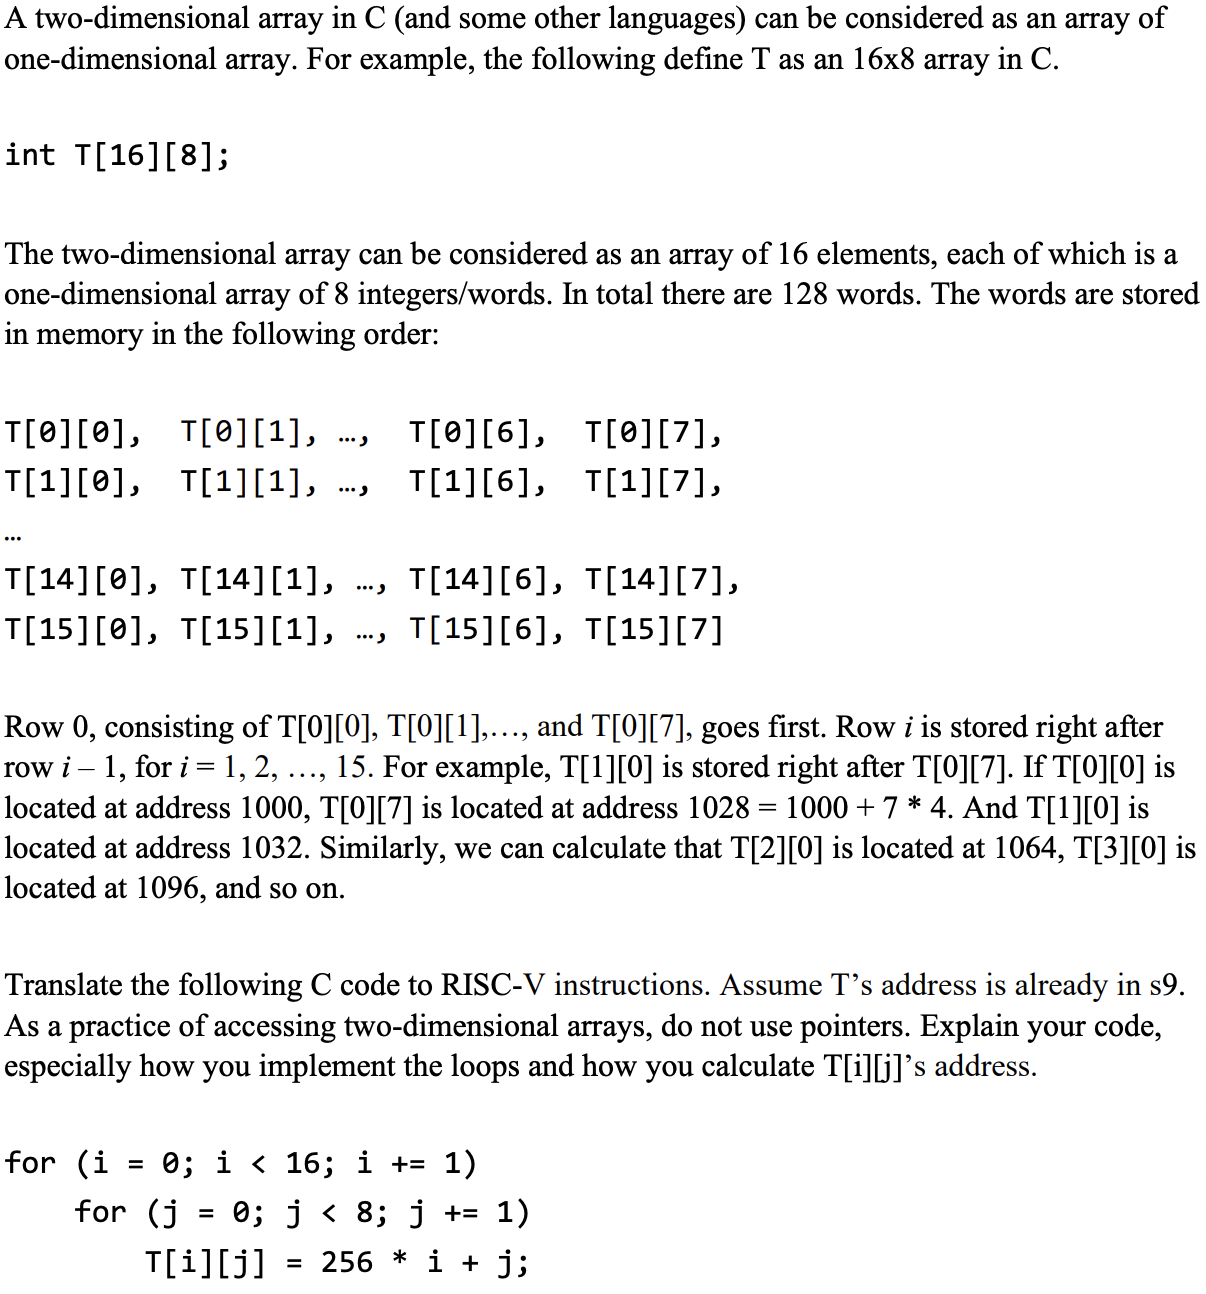
\includegraphics[scale=.534]{./images/q2Question.png}
\end{center}

\subsection*{Answer:}
The orginal C code basically has a double for loop that in
the first loop, iterates 16 times and in the second loop 8 times,
all the while setting the value T[i][j] to $256 * i + j$. The RISC-V
code works in a similar way. We first defined the values of i and the constants
like 16 and 8. We then jump to the end where the test case is and checks if
i < 16 while setting j to 0. If the test case is true, we jump to the inner
loop where we perform the operation to put in the value for $256 * i + j$.
We then find the address of T[i][j] by first computing the address of T[i] then 
adding the address for j into it. We then store the value into the address then increment
j and repeat the loop until all statments are true and executed.

\begin{lstlisting}
	# s9 = T's address

	addi	s0,s0,0 #i = 0
	addi	s2,s2,16 #16
	addi	s3,s3,8 #8
	beq	x0,x0,test

action: slli	t0,s0,256 # t0 = i * 256
	add	t0,t0,s1 # t0 + j
	
	slli	t1,s0,2 # t1 = i * 4
	slli	t2,s1,2 # t2 = j * 4
	add	t3,t1,s9 # Compute address of T[i]
	add	t3,t3,t2 # Compute address of T[i][j]
	sw	t0,0(t3) # T[i][j] = t0
	
test2:	addi	s1,s1,1 #j++
	blt	s1,s3,action #j < 8
	addi	s0,s0,1 #i++
test: 	addi	s1,x0,0 #j = 0
	blt	s0,s2,action # i < 16
\end{lstlisting}

\section*{Question 3}
\begin{center}
    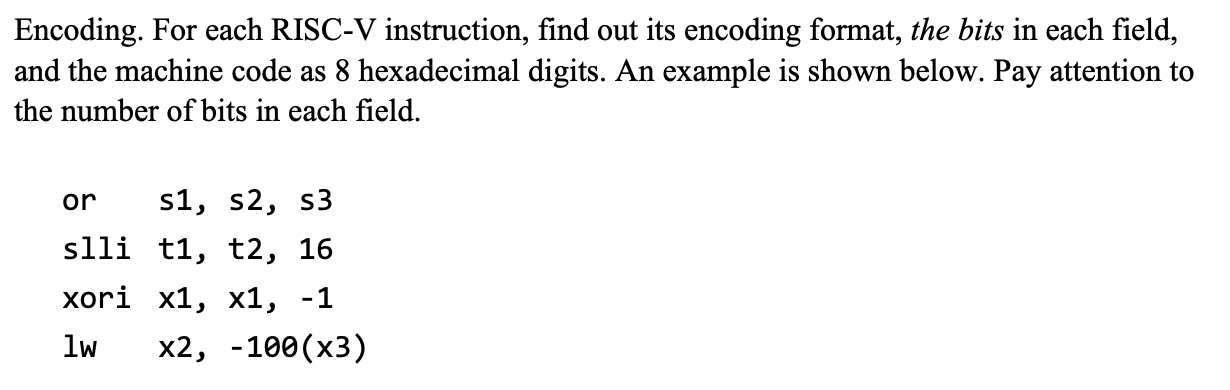
\includegraphics[scale=.559]{./images/Q3Problem.png}
\end{center}

\subsection*{Answer:}
\begin{center}
	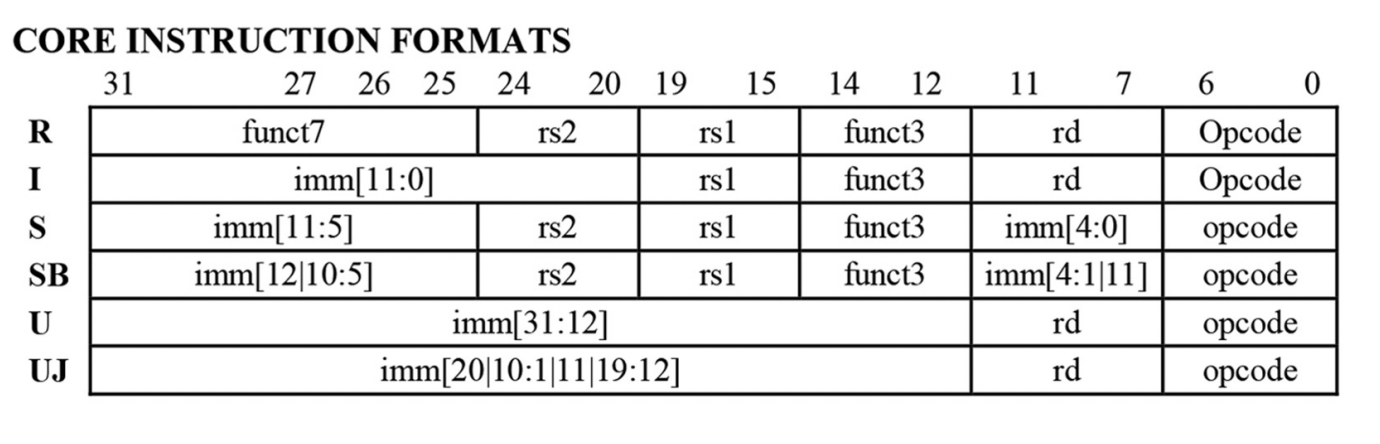
\includegraphics[scale=.45]{./images/format.png}
	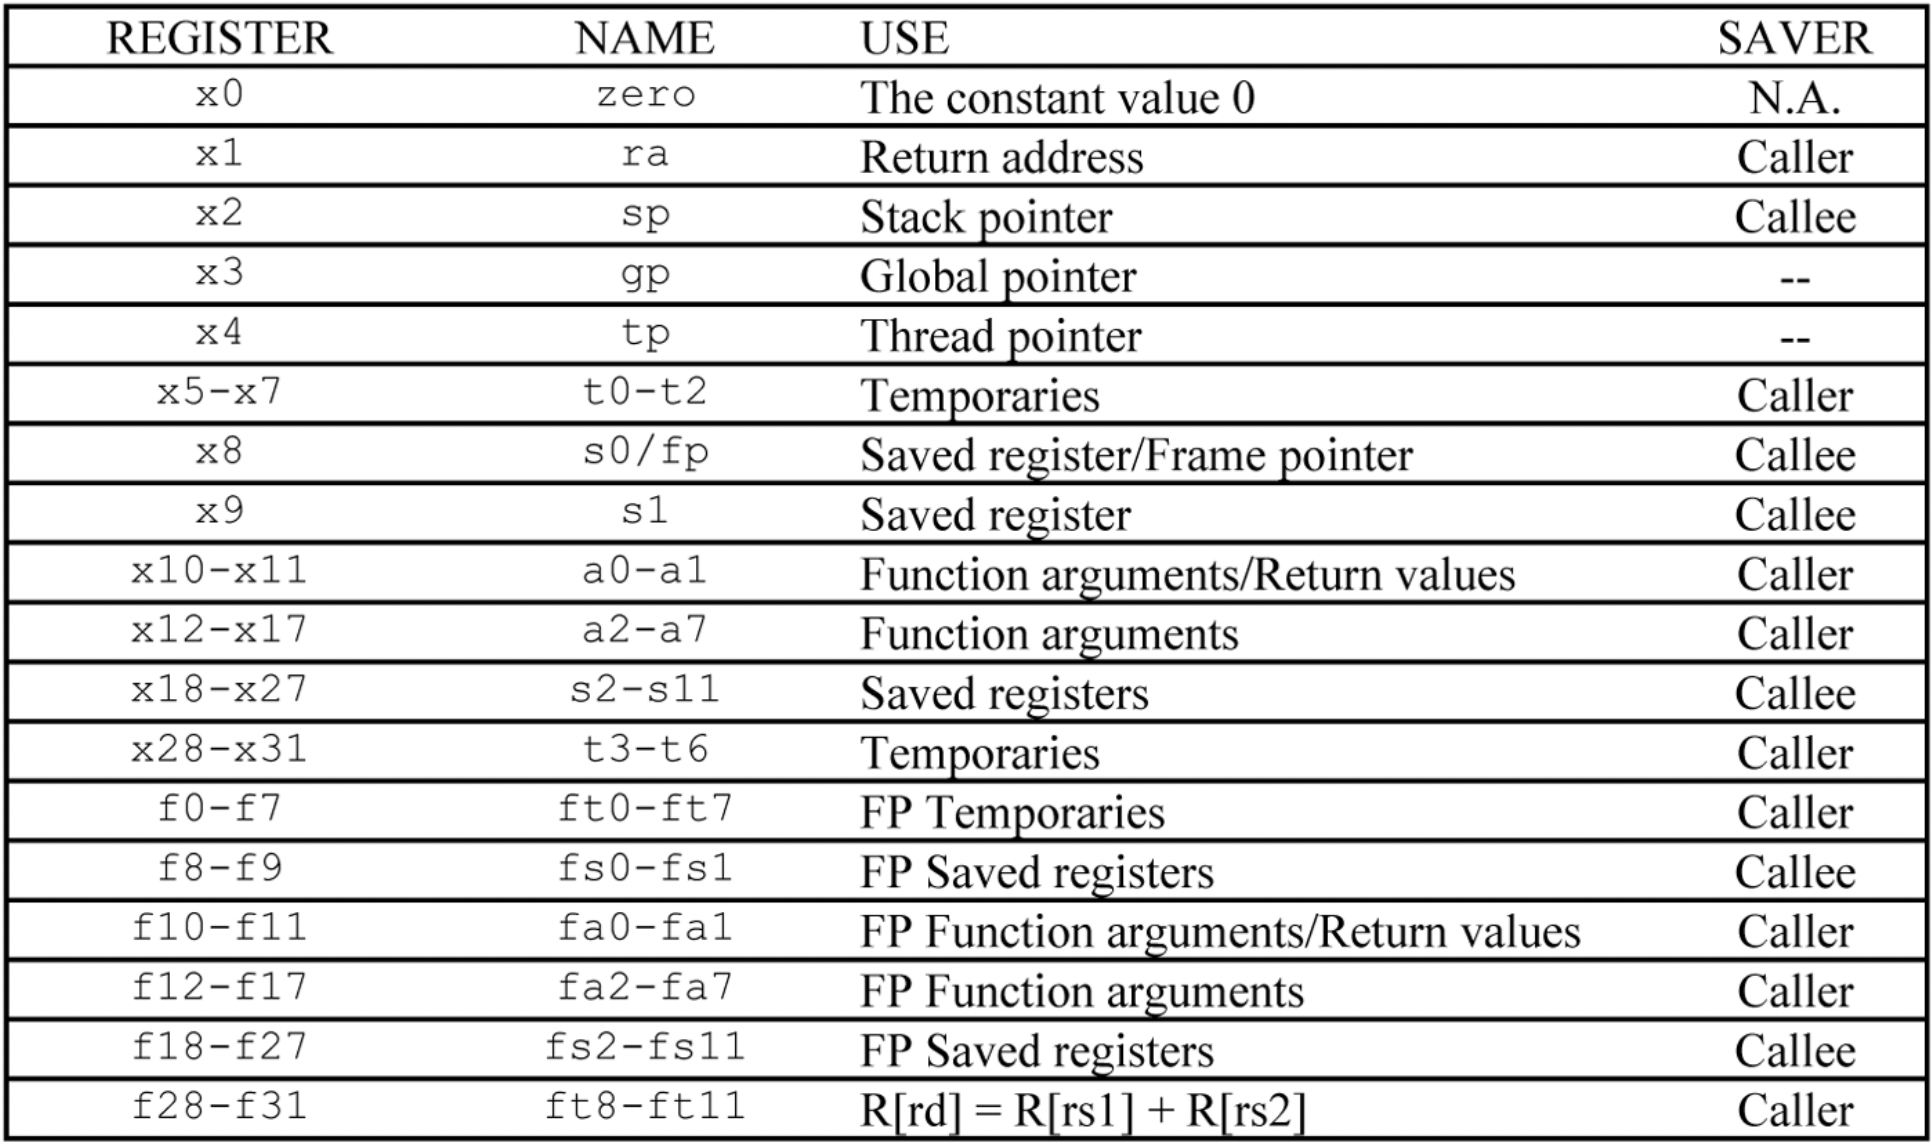
\includegraphics[scale=.3]{./images/register_list.png}
\end{center}


\subsubsection*{Instruction: or  s1, s2, s3}
Register numbers: or x9, x18, x19\\
Type: R-Type\\
opcode: 0110011\\
rd: 01001\\
funct3: 110\\
rs1: 10010\\
rs2: 10011\\
funct7: 0000000\\
Machine code in bits: 0000 0001 0011 1001 0110 0100 1011 0011\\
Machine code in hex: 0x013964B3\\

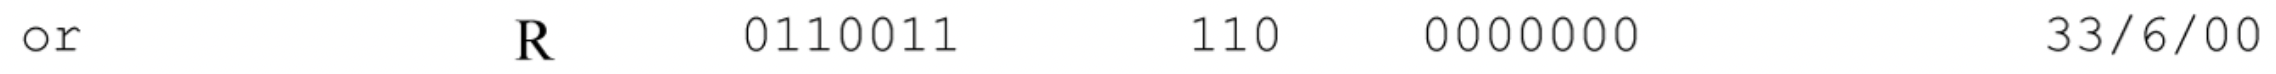
\includegraphics[scale=.25]{images/or1.png}

\begin{center}
	\begin{tabularx}{1.15\textwidth} { 
		| >{\centering\arraybackslash}X 
		| >{\centering\arraybackslash}X 
		| >{\centering\arraybackslash}X 
		| >{\centering\arraybackslash}X
		| >{\centering\arraybackslash}X
		| >{\centering\arraybackslash}X | }
	   \hline
	   	funct7 & rs2 & rs1 & funct3 & rd & Opcode \\
	   \hline
	   0000000  & 10011  & 10010 & 110 & 01001 &  0110011\\
	  \hline
	\end{tabularx}
\end{center}


\subsubsection*{Instruction: slli  t1, t2, 16}
Register numbers: slli x6,x7,16\\
Type: I-Type\\
opcode: 0010011\\
rd: 00110\\
funct3: 001\\
rs1: 00111\\
shift: 10000\\
Immediate: 0000000\\
Machine code in bits: 0000 0001 0000 0011 1001 0011 0001 0011\\
Machine code in hex: 0x1039313\\

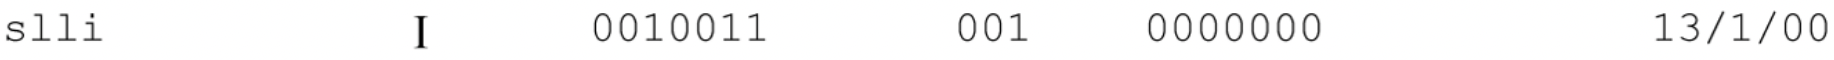
\includegraphics[scale=.35]{./images/slli1.png}

\begin{center}
	\begin{tabularx}{1.15\textwidth} { 
		| >{\centering\arraybackslash}X 
		| >{\centering\arraybackslash}X 
		| >{\centering\arraybackslash}X 
		| >{\centering\arraybackslash}X
		| >{\centering\arraybackslash}X | }
	   \hline
	   	imm[11:0] & rs1 & funct3 & rd & Opcode \\
	   \hline
	   000000010000  & 00111  & 001 & 00110 & 0010011 \\
	  \hline
	\end{tabularx}
\end{center}


\hspace{3in}

\subsubsection*{Instruction: xori  x1, x1, -1}
Register numbers: xori x1,x1,-1\\
Type: I-Type\\
opcode: 0010011\\
rd: 00001\\
funct3: 100\\
rs1: 00001\\
Immediate: 111111111111\\
Machine code in bits: 1111 1111 1111 0000 1100 0000 1001 0011\\
Machine code in hex: 0xFFF0C093\\

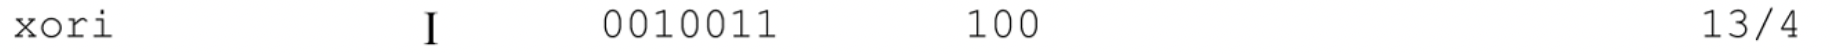
\includegraphics[scale=.35]{./images/xori1.png}

\begin{center}
	\begin{tabularx}{1.15\textwidth} { 
		| >{\centering\arraybackslash}X 
		| >{\centering\arraybackslash}X 
		| >{\centering\arraybackslash}X 
		| >{\centering\arraybackslash}X
		| >{\centering\arraybackslash}X | }
	   \hline
	   	imm[11:0] & rs1 & funct3 & rd & Opcode \\
	   \hline
	   111111111111  & 00001  & 100 & 00001 & 0010011 \\
	  \hline
	\end{tabularx}
\end{center}

\hspace{3in}

\subsubsection*{Instruction: lw  x2, -100(x3)}
Register numbers: lw x2, -100(x3)\\
Type: I-Type\\
opcode: 0000011\\
rd: 00010\\
funct3: 010\\
rs1: 00011\\
Immediate: 111110011100\\
Machine code in bits: 1111 1001 1100 0001 1010 0001 0000 0011\\
Machine code in hex: 0xF9C1A103\\

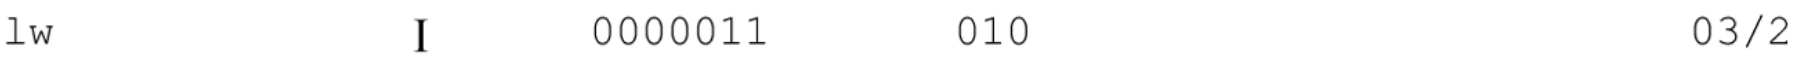
\includegraphics[scale=.35]{./images/lw1.png}

\begin{center}
	\begin{tabularx}{1.15\textwidth} { 
		| >{\centering\arraybackslash}X 
		| >{\centering\arraybackslash}X 
		| >{\centering\arraybackslash}X 
		| >{\centering\arraybackslash}X
		| >{\centering\arraybackslash}X | }
	   \hline
	   	imm[11:0] & rs1 & funct3 & rd & Opcode \\
	   \hline
	   111110011100  & 00011  & 010 & 00010 & 0000011 \\
	  \hline
	\end{tabularx}
\end{center}

\hspace{3in}

\section*{Question 4}
\begin{center}
	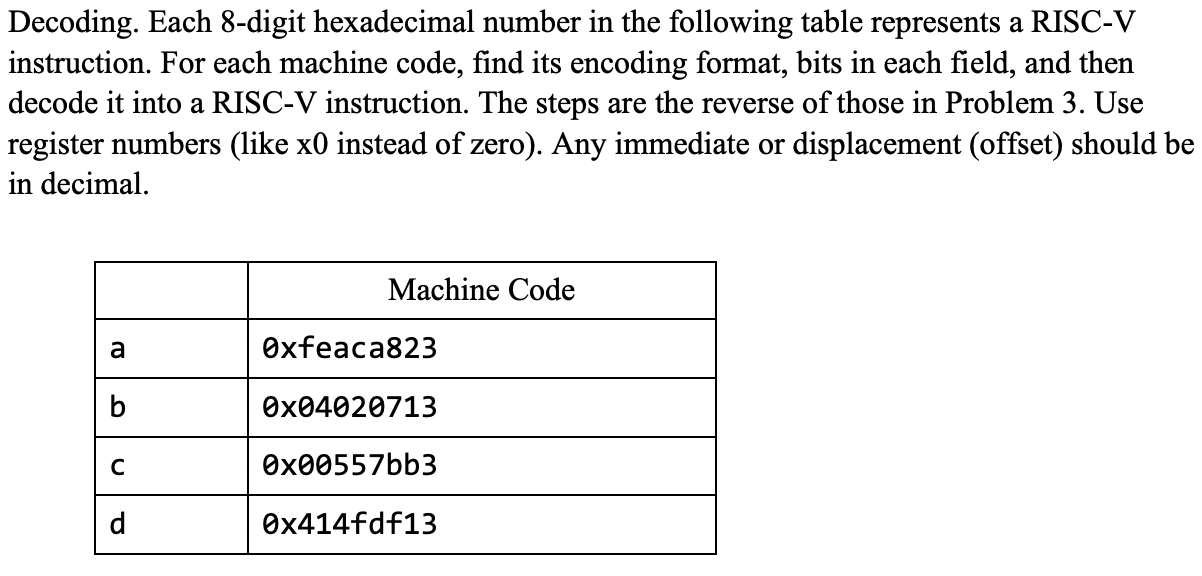
\includegraphics[scale=.572]{./images/Q4Problem.png}
\end{center}

\subsection*{Answer:}
\subsubsection*{Machine code: 0xFEACA823}

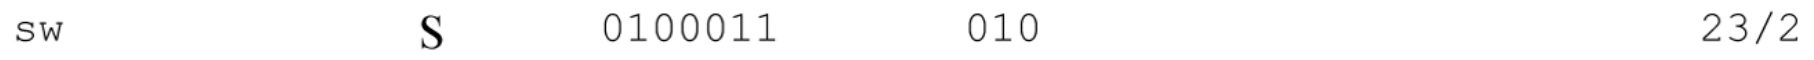
\includegraphics[scale=.3]{images/swq4.png}
\\\\
Code in bits: 1111111 01010 11001 010 10000 0100011\\
Type: S-Type\\
Opcode: 0100011 (Type S-Type)\\
Immediate1: 10000 (Decimal: 16)\\
funct3: 010 (Instruction sw)\\ 
rs1: 11001 (Decimal 25)\\
rs2: 01010 (Decimal 10)\\
Immediate2: 1111111 (Negative)\\
Translation: sw x10, -16(x25)\\

\subsubsection*{Machine code: 0x04020713}

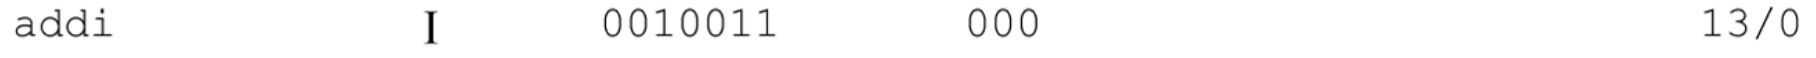
\includegraphics[scale=.3]{images/addiq4.png}
\\\\
Code in bits: 000001000000 00100 000 01110 0010011\\
Type: I-Type\\
Opcode: 0010011 (Type I-Type)\\
rd: 01110 (Decimal 14)\\
funct3: 000 (Instruction addi)\\
rs1: 00100 (Decimal 4)\\
Immediate: 000001000000 (Decimal 64)\\
Translation: addi x14, x4, 64\\

\subsubsection*{Machine code: 0x00557BB3}

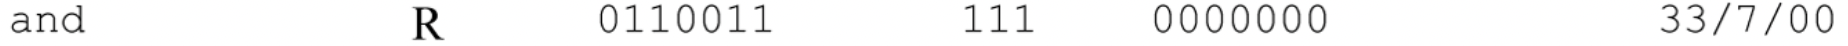
\includegraphics[scale=.3]{images/andq4.png}
\\\\
Code in bits: 0000000 00101 01010 111 10111 0110011\\
Type: R-Type\\
Opcode: 0110011 (Type R-Type)\\
rd: 10111 (Decimal 23)\\
funct3: 111 (Instruction and)\\
rs1: 01010 (Decimal 10)\\
rs2: 00101 (Decimal 5)\\
funct7: 0000000 (Decimal 0)\\
Translation: and x23, x10, x5\\

\subsubsection*{Machine code: 0x414FDF13}

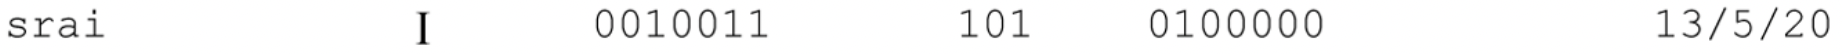
\includegraphics[scale=.3]{images/sraiq4.png}
\\\\
Code in bits: 010000010100 11111 101 11110 0010011\\
Type: I-Type\\
Opcode: 0010011 (Type I-Type)\\
rd: 11110 (Decimal 30)\\
funct3: 101 (Instruction srai)\\
rs1: 11111 (Decimal 31)\\
shift: 010100 (Decimal 20)\\
Immediate: 0100000\\
Translation: srai x30, x31, 20\\


\end{document}